\section{VLM の教師と文の埋め込みの生徒}
\label{sec_text}
本章では，発話の型と必要な知識について，規則，VLM の教師，教師ラベルで学習した文の埋め込みの分類器（生徒）を比較した経緯を述べる．

\subsection{第1版での比較}
最初の比較では，第1版の検証データ420件（最終評価用210件，当時の目視ラベル）を用いた．
規則は，形式が穴埋め・お題文なら回答とし，それ以外は括弧，文末，呼びかけの語などの手がかりで発話の型を決めた．
教師は Qwen3-VL の 8B，30B-A3B，32B であり，お題画像，形式，ボケを与えて全項目を JSON で答えさせた．
生徒は，30B-A3B が学習用のボケ3.5万件に付けたラベルで学習した MLP であり，入力はボケの文の埋め込み，お題の形式・属性・媒体，お題画像の埋め込みの組み合わせとした．

表\ref{tab_v1}に，最終評価用210件での結果を示す．

\begin{table}[t]
    \centering
    \caption{第1版の検証データ（最終評価用210件，当時の目視ラベル）での比較．発話の型と必要な知識はマクロ F1，文字は画像中の文字への依存の F1，順守はカルタ・穴埋め・お題文のボケの正解率，速度は1秒あたりの件数．第2版は教師への指示の改訂版である．生徒は3 seed の平均．}
    \label{tab_v1}
    \footnotesize
    \setlength{\tabcolsep}{2.5pt}
    \begin{tabular}{@{}lccccr@{}}
        \toprule
        方法 & 発話 & 知識 & 文字 & 順守 & 速度 \\
        \midrule
        規則 & 0.45 & 0.12 & 0.77 & \textbf{0.97} & 約4.1万 \\
        教師 8B（第1版） & 0.41 & 0.32 & 0.70 & 0.88 & 11 \\
        教師 30B-A3B（第1版） & 0.47 & 0.15 & 0.71 & 0.98 & 14 \\
        教師 30B-A3B（第2版） & 0.41 & 0.47 & 0.78 & 0.97 & 12 \\
        教師 32B（第1版） & 0.53 & 0.29 & 0.75 & 0.98 & 6 \\
        教師 32B（第2版） & \textbf{0.56} & 0.43 & 0.74 & 0.96 & 4 \\
        生徒 MLP（文） & 0.23 & 0.35 & 0.52 & 0.97 & 約40万 \\
        生徒 MLP（文＋形式） & 0.33 & 0.39 & 0.77 & 0.97 & 約40万 \\
        生徒 MLP（文＋形式＋画像） & 0.36 & 0.36 & 0.77 & 0.97 & 約39万 \\
        生徒 文の分類器の微調整 & 0.39 & 0.42 & 0.78 & 0.97 & 約3,100 \\
        目視ラベルのみ（210件） & 0.37 & 0.36 & \textbf{0.90} & 0.82 & --- \\
        生徒＋目視ラベルで補正 & 0.42 & \textbf{0.48} & \textbf{0.90} & 0.89 & --- \\
        \bottomrule
    \end{tabular}
\end{table}

この段階では，発話の型の6区分のマクロ F1 は規則が0.45，32B が0.56であり，生徒は0.23〜0.39と規則を下回った．
生徒の速度は文の埋め込みの計算を含まない値であり，埋め込みは約4,700〜9,600件/秒で計算できた．
主な原因は教師の偏りであった．
30B-A3B は学習用のボケの48\%をツッコミとし，状況の説明をほとんど付けなかったため，生徒はこの偏りを受け継いだ．
必要な知識の4段階のマクロ F1 は最高でも0.48であった．
教師は「急カーブ」「つきあい」のような一般的な語を特定の事物とし，30B-A3B は第1版の指示で知識をほぼ全て画像中のオブジェクトとした．
一方，最終評価用210件の目視ラベルで生徒の出力を補正すると（以下，補正），必要な知識と画像中の文字の精度が教師と同等以上になり，少量の目視ラベルの効果が大きいことが示された．
補正では，生徒の出力の確率とお題の特徴を入力とするロジスティック回帰を，調整用データの目視ラベルで学習して最終評価用データを予測し，逆の組み合わせも行った．

\subsection{教師ラベルの水増しと重み付き損失}
発話の型の生徒を改善するため，最も精度の高い 32B の教師で，学習用のボケ9,041件にラベルを付け直した．
内訳は，無作為の5,000件と，規則か教師が少ない型と予測した候補の約4,000件である．
さらに，型の出現回数の逆数で重みを付けた交差エントロピーで学習した．
表\ref{tab_text_students}に，検証データ620件の合意ラベルで評価した結果を示す．

\begin{table}[t]
    \centering
    \caption{規則，教師，文の埋め込みの生徒の比較（合意ラベル）．6区分と3区分はマクロ F1，画像外は「はい」の F1．生徒は3 seed の平均である．}
    \label{tab_text_students}
    \small
    \begin{tabular}{@{}lcccc@{}}
        \toprule
        & \multicolumn{2}{c}{6区分} & 3区分 & 画像外 \\
        方法 & dev & test & test & test \\
        \midrule
        規則 & 0.49 & 0.51 & 0.74 & --- \\
        教師 32B（第3版） & 0.49 & 0.53 & 0.81 & 0.32 \\
        教師 30B-A3B（第3版） & 0.44 & 0.41 & 0.72 & 0.47 \\
        生徒（水増し＋重み） & 0.54 & 0.56 & 0.81 & 0.14 \\
        生徒（水増し＋重み＋補正） & 0.58 & 0.61 & 0.81 & 0.47 \\
        教師 32B（one\_kt\_cap） & 0.56 & 0.56 & 0.79 & \textbf{0.67} \\
        生徒（one\_kt\_cap，3.5万件） & \textbf{0.65} & \textbf{0.61} & \textbf{0.82} & 0.60 \\
        \bottomrule
    \end{tabular}
\end{table}

水増しと重み付き損失により，生徒の6区分は教師を上回った．
生徒は画像を入力せず文と形式だけを用いるが，教師が状況の説明をほとんど使わない偏りを重み付き損失が打ち消したためと考えられる．
一方，ツッコミはどの方法でも F1 0.2前後であった．
教師はツッコミを多用し，水増し用の集合の33\%をツッコミとしたのに対し，目視では検証データの4\%しかない．

6区分のうち，セリフと心の声を統合した5区分ではマクロ F1 が最高0.66，さらにツッコミ・状況の説明・名付け・見立てを外からの言葉に統合した3区分では0.82であった（当時の目視ラベル）．
この結果を受けて，第3版では6区分を信頼性の低いラベルとし，3区分を併記した．

\subsection{必要な知識の判定の試み}
必要な知識の4段階を改善するため，第2版では，見た目だけで分かるか，一般常識を加えれば分かるか，画像中の対象の情報が要るか，画像外の情報が要るかを順に問う指示を教師に与えた．
しかし，順に問うと最初の問いに真と答えやすくなり，見た目だけに偏ったため，4段階のマクロ F1 は32B で0.42，30B-A3B で0.37にとどまった．
また，固有名詞の割合などの品詞の特徴34次元を形態素解析で作り，生徒の入力に加えたが，効果はなかった．
固有名詞を含まない有名な台詞の引用や，固有名詞を含んでも画像中の対象の名前であるボケが多いことと，形態素解析の辞書が漫画やタレントの名前を固有名詞と判定しないことが原因であった．
表\ref{tab_text_students}の教師 32B（第3版）の画像外の F1 は，この順に問う指示で「画像外」と判定された項目を「はい」とみなした値であり，再現率が低い．

\subsection{教師の指示の比較}
第3版の定義に合わせて，32B の教師への指示を6通りに書き直し，調整用データで比較した．
6通りは，第3版の手順を示して6区分から1つを選ばせ，画像外の知識を1つの真偽で問う指示（one），one に写真のキャプションと媒体・文字の有無を文で加えた指示（one\_cap），one\_cap の画像外の知識の問いを，依存する事物とその種類（作品，人物，商品，地名，出来事，ボケての慣習，一般，なし）を選ばせる問いに替えた指示（one\_kt\_cap），発話の型を話し手・名付けか・声に出すか・説明かの別の問いに分解し規則で6区分にする指示（dec），dec に13の例を加えた指示（dec\_fs）である．
図\ref{fig_teacher_prompts}に結果を示す．

\begin{figure}[t]
    \centering
    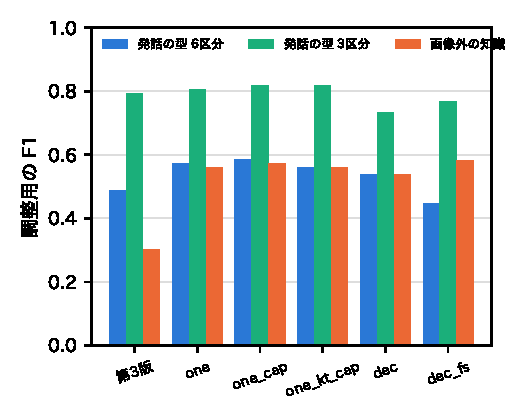
\includegraphics[width=\linewidth]{figures/fig_teacher_prompts.pdf}
    \caption{教師（Qwen3-VL-32B）の指示ごとの調整用データでの F1（合意ラベル）．第3版は4段階を順に問う指示，他は第3版の定義に合わせて書き直した指示である．}
    \label{fig_teacher_prompts}
\end{figure}

手順を書き込んで1つを選ばせる one は，第3版の指示より6区分が0.49から0.57に上がり，キャプションを加えた one\_cap で0.58となった．
一方，問いの分解は6区分をかえって下げた．
分解した指示では，モデルが話し手を「画像を見ている人」と答える偏りがあり，セリフ211件のうち134件がツッコミになった．
話し手の既定を画像の中の誰かとするよう問い直しても，最終評価用では one に及ばなかった．
例示も発話の型をツッコミに寄せた．
画像外の知識では，依存する事物の種類を選ばせる one\_kt\_cap が，普通名詞を特定の事物とする誤りを減らし，最終評価用で F1 0.67と最も高かった．
以上から，教師は one\_kt\_cap とし，学習用のボケ3.5万件（水増し用の9,041件と，他の学習用のボケ25,593件）に付け直した．
このラベルで学習した文の生徒は，6区分で調整用0.65，最終評価用0.61，画像外の知識で0.60となった．

文の生徒は，文の埋め込みの計算を含めても全件を短時間で処理できる．
しかし，画像外の知識では教師との差が大きく，画像に写っている対象と画像外の事物を区別するには画像の情報が要ると考えられた．
次章では，お題画像とボケの両方を入力とする VLM を生徒とする．
